\documentclass[12pt, twocolumn]{article}
\usepackage[utf8]{inputenc}
\usepackage{amsmath}
\usepackage[margin = 1.1in]{geometry}
\usepackage{float}
\usepackage{graphicx}
\graphicspath{{images/}}
\setlength{\columnsep}{0.75cm}
\usepackage{hyperref}
\newcommand{\solution}{\noindent \textbf{Solution: }}
\usepackage{tfrupee}
\hypersetup{
colorlinks=true,
    linkcolor= red,
    }

\title{AI1110 Assignment 1}
\author{JARUPULA SAI KUMAR CS21BTECH11023}
\date{May 2022}

\begin{document}
\maketitle
\begin{problem}
\textbf{Q7(B):} On a map drawn to a scale of 1 : 50,000, a rectangular plot of land ABCD has the
following dimensions. AB = 6cm; BC = 8cm and all angles are right angles. Find:
(i) the actual length of the diagonal distance AC of the plot in km.
(ii) the actual area of the plot in sq km.
\end{problem}

\solution 
According to given question

Given Scale 1:50,000

1 Cm Represents 50,000 cm =\cdot\frac{50,000}{1000\cdot100}=0.5Km

\implies(1) \text{In} $\Delta{}$ABC 

By applying Pythogoras Theorem
\begin{align}
\implies AC^2 &= AB^2+BC^2\\
\implies AC^2 &= 6^2+8^2\\
\implies AC^2 &=36+64
\end{align}
Finally we get AC= 10 cm\\

\implies length  of diagnol of AC=10\cdot0.5=5Km


\implies(2) We Know that,
Area of Rectangle ABCD=AB\cdot BC

=6\cdot8=48cm^2\\
Actuall Plot of Area = 48\cdot 0.25=12 km^2\\

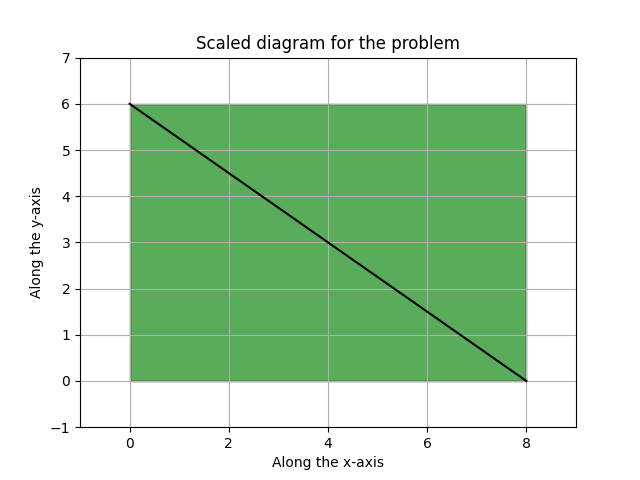
\includegraphics[width=\columnwidth]{Figure_1.1.png}
\end{document}
